\chapter{Introducción} 
\section{Los problemas clásicos de levantamiento: extensión y clasificación}
En distintos contextos matemáticos encontramos dos problemas básicos, común a todos ellos, si los despojamos de las características propias de un entorno: los problemas de extensión y levantamiento. \par

\subsection*{El problema de la extensión} 
Dado un diagrama de aplicaciones continuas 
$$
\begin{tikzcd}
	A \rar{f} \dar[hook]{i} & Y \\
	X \urar[dashed]{\tilde{f}}	&
\end{tikzcd} 
$$
donde $i$ es una ``inclusión'' en un contexto dado, ¿cuándo existe $\tilde{f}$, extensión de $f$? \par

La respuesta no es trivial. Es claro que, incluso si $i$ no es inclusión, ha de verificarse que si $i(a)= i(b)$ entonces $f(a) = f(b)$. Pero incluso si $i$ es biyectiva es necesario exigirle a $X$, para que la única $\tilde{f}$ posible sea continua, que posea la topología de la identificación determinada por $i$: 
$$
\theta \subset X \text{ es abierto si y sólo si } i^{-1} (\theta) \text{ es abierto de } A. 
$$
\newpage
Hay varios ejemplos de resultados que dan respuesta a este problema. Algunos dan una respuesta positiva:
\begin{teor} 
Si $X,Y$ son espacios métricos, $Y$ completo, y $A$ es denso en $X$, toda aplicación uniformemente continua $f:A\rightarrow Y $ se extiende a una uniformemente continua $\tilde{f} : X \rightarrow Y$.
\end{teor} 

\begin{teor}[de Extensión de Tietze]
Sea $X$ normal, $A \subset X$ cerrado, $I \subset \mathbb{R}$ intervalo. Entonces toda $f : A \rightarrow I $  admite una extensión $\tilde{f} : X \rightarrow I$.
\end{teor}
Mientras que la de otros es negativa:
\begin{teor} 
La esfera $S^{n}$ no es un retracto del disco $D^{n+1}$. En otras palabras la identidad $S^{n} \rightarrow S^{n}$ no se extiende a $D^{n+1}$.
\end{teor}

\subsection*{El problema del levantamiento}
Dualmente \footnote{Dual en el sentido de ``Eckmann-Hilton'', dualidad que se definirá más adelante.},
nos encontramos con el problema del levantamiento de aplicaciones continuas. Es el siguiente: dado un diagrama
$$
\begin{tikzcd}
	{}	& X \dar[two heads]{p} \\
	Y \urar[dashed]{\tilde{f}} \rar{f} & B
\end{tikzcd}
$$
donde $p$ es sobreyectiva ¿cuándo existe $\tilde{f}$, levantamiento de $f$?\\ 
La respuesta tampoco es elemental. Incluso si $p$ es biyectiva hay que exigirle que sea homeomorfismo para que la única $\tilde{f}$ sea continua.\par

Igualmente hay resultados clásicos en distintos ambientes que contestan parcialmente esta cuestión.

\begin{teor} 
Sea $A \subset \mathbb{R}^2$ un conjunto estrellado respecto a $x_{0} \in A$ y $f : A \rightarrow S^{1}$ una aplicación continua. Entonces f queda determinada de forma continua por su función angular, esto es, existe una aplicación $\tilde{f} : A \rightarrow \mathbb{R}$ de tal forma que el siguiente diagrama es conmutativo:
$$
\begin{tikzcd}
	{}	& \mathbb{R} \dar{exp} \\
	A \urar{\tilde{f}} \rar{f} & S^1
\end{tikzcd}
$$
Esto es, $f(x) = (cos\tilde{f}(x), sen\tilde{f}(x))$. Es más, dos tales funciones $\tilde{f}$ se diferencian en un múltiplo entero de $2\pi$.
\end{teor}

Estos problemas son, en parte, origen de la teoria de homotopía. Muchas veces, los problemas de extensión y levantamiento son puramente homotópicos: \par

Hay aplicaciones $p : X \rightarrow B$ para las que existe el levantamiento de $f : Y \rightarrow B$ si existe el levantamiento de una ``deformada'' de $f$. \par
De igual forma existen algunas aplicaciones $i : A \rightarrow X$ para las que existe una extensión de $g : A \rightarrow Y$ si y sólo si existe alguna extensión para una ``deformada'' de g. \par

Introduzcamos el concepto de deformación en homotopía:
\begin{defin}
Dos aplicaciones $f, g : X \rightarrow Y$ se dicen homótopas (deformables la una en la otra), denotado por $f \simeq g$, si existe  $H : X \times [0,1] \rightarrow Y$ una aplicación tal que $H(x ,0) = f(x)$ y $H(x, 1) = g(x)$.
\end{defin}
Llegados a este punto, los problemas de extensión y levantamiento deparan ahora a un problema común de clasificación. ¿Cuándo dos aplicaciones $X \rightarrow Y$ son homótopas? ¿Cómo es el conjunto $[X, Y]$ de clases de homotopía de aplicaciones $X \rightarrow Y$? \par 
Los métodos que se siguen son, a grosso modo, de dos enfoques distintos:\\
Por una parte, a los espacios se le asocian modelos algebraicos y morfismos entre los respectivos modelos algebraicos a las aplicaciones. Estas asociaciones permiten parcialmente su clasificación. \par 
Como ejemplo, probemos el teorema anterior por el que $S^n$ no es un retracto de $D^{n+1}$. Para ello, asociemos a $S^n$ un invariante algebraico no nulo. Como el disco $D^{n+1}$ es deformable a un punto, todos esos invariantes se hacen 0. Si $S^n$ fuese retracto de $D^{n+1}$ existiría un diagrama como el siguiente:
$$
\begin{tikzcd}
	S^n \arrow{rr}{Id_{S^n}} \drar{i} & & S^n \\
		&	D^{n+1} \urar{r} & 
\end{tikzcd}
$$
que algebraicamente daría lugar a 
$$
\begin{tikzcd}
	0 \neq F(S^n) \arrow{rr}{Id} \drar & &  F(S^n) \neq 0 \\
		&	0 \urar & 
\end{tikzcd}
$$
lo que resulta contradictorio. \par

Por otra parte, para saber más sobre $[X, Y]$ es habitual tratar de dotar a este conjunto de otras estructuras (grupo, módulo...) que den luz sobre un comportamiento. \par 



\section{Homotopía: Nociones básicas}
La relación de homotopía es básica y formaliza la noción de deformación continua de dos espacios: dos aplicaciones $f, g : X\rightarrow Y$ son homótopas si existe $H:X\times I \rightarrow Y$ tal que $H(x, 0) = f(x)$, $H(x, 1) = g(x)$. 
\begin{prop}
La relación de homotopía es una relación de equivalencia en el conjunto de aplicaciones continuas de $X$ a $Y$.
\end{prop}
\begin{demo} 
La propiedad reflexiva es clara sin más que tomar la aplicación $F(x,t) = x$.\\
Para la simétrica, si $H : f \simeq g$ entonces $F : X \times I \rightarrow Y$, $F(x, t) = H(x, 1-t)$ es una homotopía de $g$ a $f$.\\
Veamos ahora la transitiva. Si $F : f \simeq g$, $H : g \simeq h$ entonces $G : X \times I \rightarrow Y$,

$$G(x, t) = 
\begin{cases}
	F(x, 2t) 	& 	\text{ si } t \leq \frac{1}{2}\\
	H(x, 2t - 1)& 	\text{ si } t \geq \frac{1}{2}
\end{cases}$$ 
es una homotopía de $f$ a $h$.
\end{demo}
\begin{ejems}
\begin{itemize}
\item[(1)] Cuando $X = I$, esto es, al trabajar con curvas, se observa mejor la deformación:
\begin{figure}[h]
\centering
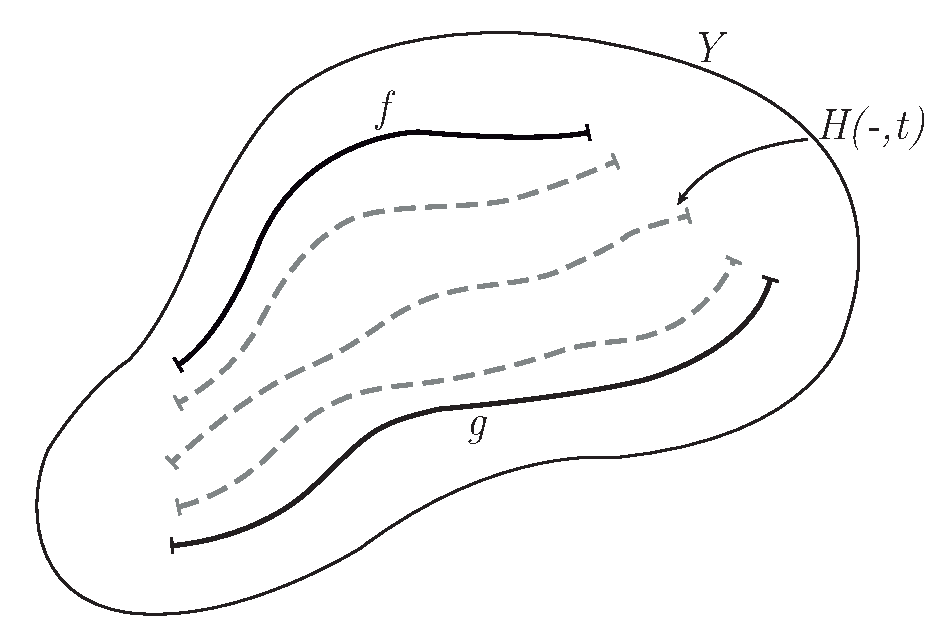
\includegraphics[width=7cm]{images/pag8.pdf}
\end{figure}
\item[(2)] Sean $X = Y = \mathbb{R}^n$, y consideremos las aplicaciones $f = 1_{\mathbb{R}^n}$ y $g \equiv 0$. Entonces $f \simeq g$ mediante la aplicación
$$H : \mathbb{R}^n \times I \rightarrow \mathbb{R}^n$$ $$H(x, t) = tx$$
\end{itemize}
\end{ejems}
A menudo estamos interesados en aplicaciones entre pares
$$f : (X, A) \rightarrow (Y, B)$$ que no es más que una aplicación continua tal que $f(A) \subset B$. En este caso, $f, g : (X, A) \rightarrow (Y, B)$ son homótopas si existe $H : X \times I \rightarrow Y$ tal que $\forall t \in I$, $H_t = H(-, t) : (X, A) \rightarrow (Y, B)$.\footnote{Arreglar, explicar}\\
Un caso particular de suma importancia es el de los espacios punteados $(X, x_0)$. En este caso, $f \simeq g : (X, x_0) \rightarrow (Y, y_0)$ si existe $H: X \times I \rightarrow Y$ tal que $H(x, 0) = f(x), H(x, 1) = g(x)$ y $H(x_0, t) = y_0$ $\forall t \in I$.\\
\begin{ejems}
\begin{itemize}
\item[(1)] En el ejemplo anterior (2), podemos considerar $f \simeq g : (\mathbb{R}^n, 0) \rightarrow (\mathbb{R}^n, 0)$ tomando como homotopía la misma función $H$.
\item[(2)] Si consideramos un espacio como el siguiente: \textbf{(Insertar imagen p9)} Tenemos que $f : I \rightarrow Y$ es obviamente homótopa a la constante en $y_0$ que denominamos $c_{y_0}$. Pero la aplicación de pares $f : (I, \{ 0,1 \} \rightarrow (Y, y_0)$ no es homótopa a la constante $c_{y_0}$.
\item[(3)] Dado $E^2 = \{ x \in \mathbb{R}^2 : \| x \| \leq 1 \}$, tenemos que $1 \simeq a$ donde $a$ es la función antípoda mediante la hopotopía de la rotación: $H : E^2 \times I \rightarrow E^2$ dada por $H(x, t) = H(\rho e^{i\theta}, t) = \rho e^{i(\theta + t\pi)}$ \textbf{(Insertar gráfico p10)}\\
Es más, como aplicaciones de pares, $1 \simeq a$ mediante $H : (E^2, S^1) \times I \rightarrow (E^2, S^1)$. Sin embargo, $\nexists x_0 \neq 0$ tal que $1 \simeq a$ como aplicaciones $(E^2, x_0) \rightarrow (E^2, -x_0)$.
\end{itemize}
\end{ejems}
Al conjunto cociente formado por las clases de homotopía de aplicaciones continuas de $(X, A)$ en $(Y, B)$ se le denota por $[(X, A), (Y, B)]$.\\
Por tanto, ya podemos definir nuestros ``objetos de plastilina''.
\begin{defin}
Dos espacios $X$ e $Y$ son homotópicamente equivalentes si existen aplicaciones $f: X \rightarrow Y$ y $g: Y \rightarrow X$ tales que $g \circ f \simeq 1_X$ y $f \circ g \simeq 1_Y$ \\
A las aplicaciones $f$ y $g$ se les denomina equivalencias de homotopía.
\end{defin}

\begin{ejems}
\begin{itemize}
\item[(1)] \textbf{Retractos}: 
\begin{tikzcd}
A \rar[hook]{i} & X  
\end{tikzcd}
es un retracto de X si existe una aplicación $r : X \rightarrow A$ tal que $r \circ i = 1_A$.
Decimos que $A$ es un retracto de deformación de $X$ si además $i \circ r \simeq 1_X$.\\
Como ejemplo, $S^n = \{ x \in \mathbb{R}^{n+1}$ : $\| x \| = 1 \}$ es un retracto de deformación de $\mathbb{R}^{n+1} -\{ 0 \}$. En efecto, si consideramos 

$$r : \mathbb{R}^{n+1} -\{ 0 \} \rightarrow S^n $$
$$x \mapsto \frac{x}{\| x \|}$$


entonces 
$$H : \mathbb{R}^{n+1} -\{ 0 \} \times I \rightarrow \mathbb{R}^{n+1} -\{ 0 \}$$
$$H(x, t) = (1 - t)x + \frac{tx}{\| x \|}$$ es una homotopía entre $1_{\mathbb{R}^{n+1} -\{ 0 \}}$ y $i \circ r$.
\item[(2)] \textbf{Espacios contráctiles}: Un espacio X es contráctil si tiene el mismo tipo de homotopía de un punto, o equivalentemente, la identidad en $X$ es homótopa a una constante, o un punto es retracto de deformación del espacio. Antes hemos visto que $\mathbb{R}^n \simeq \ast \simeq D^n $.
\item[(3)] El espacio peine P es un espacio contráctil. \textbf{(Insertar imagen p12)}\\
$$P = \bigcup_{n=1}^\infty \left( \left\lbrace \frac{1}{n} \right\rbrace \times [0, 1]\right) \cup \{ 0 \} \times [0, 1] \cup [0, 1] \times \{ 0 \}$$ 
que obviamente es contráctil, aunque $1_p \not \simeq_{p_0} c_{p_0}$.
\end{itemize}
\end{ejems}
Relacionado con el ejemplo $(2)$ y con el problema de la extensión tenemos el siguiente resultado:\\
\begin{teor}
Sea $f : S^n \rightarrow X$ una aplicación continua. Entonces $f \simeq \ast$ si y sólo si $f$ se extiende al disco. \textbf{(Insertar diagrama p11)}
\end{teor}
\begin{demo}
Supongamos $H : f \simeq c_{x_0}$. Definimos $\tilde{f} : E^{n+1} \rightarrow X$\\
$\tilde{f}(p )= 
\begin{cases}
	x_0$ si $\| p \| \leq \frac{1}{2} \\
	H(\frac{p}{\| p \|}, 2 - 2\| p \|) si \| p \| \geq \frac{1}{2}
\end{cases}$\\
Recíprocamente, si $\tilde{f}$ es una extensión, $H(x, t) = \tilde{f}((1 - t)x)$ es una homotopía de $f$ a la constante.
\end{demo}
